\documentclass[12pt,a4paper]{report}

%% ============================================================
%%  Package Imports & Configuration
%% ============================================================
\usepackage[margin=1in]{geometry}
\usepackage[utf8]{inputenc}
\usepackage[T1]{fontenc}
\usepackage{amsmath}
\usepackage{amssymb}
\usepackage{graphicx}
\usepackage{booktabs}
\usepackage{array}
\usepackage{longtable}
\usepackage{multirow}
\usepackage{caption}
\usepackage{subcaption}
\usepackage{float}
\usepackage{cite}
\usepackage{microtype}
\usepackage{setspace}
\usepackage{titlesec}
\usepackage{fancyhdr}
\usepackage{tocloft}
\usepackage{listings}
\usepackage{xcolor}
\usepackage[hidelinks]{hyperref}
\usepackage{xurl} % Allows breakable URLs and paths anywhere
\urlstyle{same}   % Uses same font for URLs/paths as text/tt
\emergencystretch=3em % Prevents line overfull in narrow/code paragraphs

\usepackage{tikz}
\usetikzlibrary{positioning, arrows.meta, shapes.geometric}

%% ============================================================
%%  Page Style
%% ============================================================
\pagestyle{fancy}
\fancyhf{}
\renewcommand{\chaptermark}[1]{\markboth{\thechapter.\;#1}{}}
\lhead{\small\nouppercase{\leftmark}}
\rhead{\small\textit{IASc SRFP 2026}}
\cfoot{\thepage}
\setlength{\headheight}{14.5pt}
\addtolength{\topmargin}{-2.5pt}

\onehalfspacing

%% ============================================================
%%  Code listing style
%% ============================================================
\lstset{
  basicstyle=\ttfamily\footnotesize,
  breaklines=true,
  frame=single,
  language=Python,
  keywordstyle=\color{blue},
  commentstyle=\color{gray},
  stringstyle=\color{teal}
}

%% ============================================================
%%  Title & Metadata
%% ============================================================
\title{}
\date{}
\author{}

\begin{document}

%% ============================================================
%%  OFFICIAL IISC STYLE TITLE PAGE
%% ============================================================
\begin{titlepage}
  \hypersetup{pageanchor=false} % Prevents duplicate page 1 warning in hyperref
  \begin{center}

    \vspace*{-0.5cm}

    % MAIN TITLE
    {\Large \bfseries Multimodal Vision-Based PCB Reverse Engineering for Hardware Assurance} \\[14pt]

    \vspace*{0.5cm}

    % FULFILLMENT STATEMENT & PROGRAMME
    {\normalsize A Technical Internship Report Submitted in Partial Fulfillment of the Requirements} \\
    {\normalsize for the Summer Research Fellowship Programme (SRFP 2026)} \\
    \vspace{2mm}
    {\normalsize jointly offered by} \\
    \vspace{3mm}
    {\large \bfseries IASc -- INSA -- NASI} \\[6mm]
    {\em\large by} \\[6mm]
    {\large \bfseries SEIKH SOUVAGYA MUSTAKIM} \\
    {\normalsize \bfseries Application ID: ENGS5100} \\[0.4in]

    % IISC MASTER SEAL / CREST IMAGE
    \begin{center}
      \IfFileExists{Images/others/IISc_Master_Seal.jpg}{%
        \includegraphics[height=42mm]{Images/others/IISc_Master_Seal.jpg}%
      }{%
        \IfFileExists{IISc_Master_Seal.jpg}{%
          \includegraphics[height=42mm]{IISc_Master_Seal.jpg}%
        }{%
          \IfFileExists{iisc_seal.png}{%
            \includegraphics[height=42mm]{iisc_seal.png}%
          }{%
            \vspace{0.2cm}%
            \setlength{\fboxsep}{8pt}%
            \framebox[45mm]{\vbox to 35mm{\vfill\centering\bfseries\Large IISC SEAL\vfill}}%
            \vspace{0.2cm}%
          }%
        }%
      }
    \end{center}

    \vspace{0.3cm}

    % GUIDANCE & DEPARTMENT METADATA
    {\em\large under the guidance of} \\[6pt]
    {\bfseries\large DR. HARESH DAGALE} \\[8pt]
    {\bfseries\large DEPARTMENT OF ELECTRONIC SYSTEMS ENGINEERING} \\[5pt]
    {\bfseries\large INDIAN INSTITUTE OF SCIENCE} \\[5pt]
    {\bfseries\large BENGALURU -- 560012, INDIA} \\[0.4in]

    % DATE
    {\bfseries\large JULY 2026}

  \end{center}
  \hypersetup{pageanchor=true}
\end{titlepage}




%% ============================================================
%%  ACKNOWLEDGEMENTS
%% ============================================================
\newpage
\chapter*{Acknowledgements}
\addcontentsline{toc}{chapter}{Acknowledgements}

The author wishes to express sincere gratitude to the Indian Academy of Sciences (IASc) for providing the Summer Research Fellowship that made this work possible. Deep appreciation is extended to the research guide, Dr. Haresh Dagale, and the broader research community at the Department of Electronic Systems Engineering (DESE), IISc Bengaluru, for their intellectual guidance and access to computational resources throughout the fellowship period. The author also acknowledges the open-source contributions of the Ultralytics YOLOv8 team, the Roboflow annotation community, and the Schutzwerk security research group, whose publicly available datasets and implementations formed foundational principles of this work.

\newpage

%% ============================================================
%%  EXECUTIVE SUMMARY (ABSTRACT)
%% ============================================================
\begin{abstract}
\addcontentsline{toc}{chapter}{Executive Summary}

The globalization of electronics manufacturing has introduced compounding vulnerabilities across the semiconductor supply chain, enabling hardware adversaries to insert malicious logic modifications --- commonly termed hardware Trojans --- into integrated circuits or printed circuit board (PCB) assemblies without detection. Traditional PCB reverse engineering, which forms the primary auditing mechanism to identify such modifications, is constrained by a fundamental operational dichotomy: destructive acid-based chemical de-layering of substrate materials is hazardous and renders boards permanently non-functional, while contact-based robotic probing systems such as PROBoter require expensive hardware calibration and risk mechanical damage to delicate surface-mount device (SMD) pin pads. Neither paradigm scales to the forensic auditing of active, deployed equipment.

This report presents \textbf{PCBRE}, an automated, non-destructive, photograph-only pipeline for PCB reverse engineering and hardware assurance. The system integrates classical computer vision segmentation with deep learning based oriented object detection and Large Multimodal Model (LMM) driven text extraction, all coordinated through a responsive Flask web application. The pipeline operates in four sequential stages. Stage 1 applies dynamic Hue-Saturation-Value (HSV) morphological masking to isolate IC component bodies from the board substrate. Stage 2 performs text image enhancement via Contrast Limited Adaptive Histogram Equalization (CLAHE) and Gaussian Unsharp Masking to recover degraded laser-etched package markings. Stage 3 represents the central contribution: a custom-trained YOLOv8 Oriented Bounding Box (OBB) detector that achieves orientation-invariant component localization. Three model architectures --- Nano, Small, and Medium --- were trained at image resolutions of 640 and 1024 pixels. The YOLOv8m-OBB configuration, trained with 26.4 million parameters at \(1024 \times 1024\) resolution, achieves a mean Average Precision (mAP@0.5) of \textbf{0.749}, representing a \textbf{30.4\%} improvement over horizontal bounding box baselines and confirming that high-resolution inputs are critical for detecting sub-millimeter passive components. Stage 4 introduces a probe-free power rail localization framework that couples Gemini 1.5 Flash Large Multimodal Model (LMM) silkscreen parsing with local Euclidean Distance Transform width heuristics to classify VCC and GND power nets directly from image data, without physical electrical contact or access to CAD netlist files. The complete system compiles a structured Hardware Bill of Materials (HBoM) in JSON format, exportable as a CSV, covering part numbers, manufacturers, component categories, pin counts, and power topology annotations. The prototype is evaluated across five reference PCB targets including the Schutzwerk STM32F745 security board, with Gemini 1.5 Flash achieving near-perfect read accuracy on laser-etched IC package text where all local OCR engines failed.

\end{abstract}

\newpage

%% ============================================================
%%  TABLE OF CONTENTS
%% ============================================================
\tableofcontents
\newpage

%% ============================================================
%%  LIST OF FIGURES
%% ============================================================
\listoffigures
\newpage


%% ============================================================
%%  CHAPTER 1: INTRODUCTION
%% ============================================================
\chapter{Introduction}
\label{chap:introduction}

\section{Overview \& Domain Context}
\label{sec:hw_assurance}

The modern semiconductor supply chain is a globally distributed, multi-tier network that spans design houses, silicon foundries, packaging facilities, and assembly subcontractors across dozens of geopolitical boundaries. A single smartphone processor may be designed in Silicon Valley, fabricated in Taiwan, packaged in Malaysia, assembled in Shenzhen, and distributed through European logistics hubs before reaching an end consumer. This extended chain creates multiple high-value opportunities for adversarial interference. Hardware Trojans --- malicious circuits embedded within legitimate ICs or PCB interconnects --- represent one of the most technically sophisticated attack vectors in this threat landscape. Unlike software malware, hardware Trojans operate at the silicon or board level, rendering conventional software-based detection entirely ineffective.

Printed Circuit Board (PCB) reverse engineering is the systematic process of reconstructing a board's component topology, electrical netlist, and logic functions from physical inspection. It is the foundational technique in hardware assurance audits, IP protection litigation, and end-of-life component analysis. In security contexts, it enables analysts to verify that a fielded board matches its approved design files, revealing any unauthorized component substitutions or trace modifications. The output of this process is a Hardware Bill of Materials (HBoM) --- a structured catalogue of every active and passive component on the board --- and, ideally, a reconstructed schematic or netlist mapping the electrical connections between those components.

\section{Motivation}
\label{sec:motivation}

Classical PCB reverse engineering has historically relied on physical and chemical techniques that permanently destroy the sample. Chemical de-layering, in which successive board layers are dissolved using concentrated nitric or hydrofluoric acid, allows inspection of internal copper routing but precludes any further analysis of the same board and generates toxic byproducts requiring specialized disposal. X-ray tomography avoids chemical destruction but requires access to industrial CT scanner infrastructure, with reconstruction costs per board frequently exceeding \$5,000 USD. Contact-based robotic probing, as exemplified by the PROBoter system from Schutzwerk GmbH, automates electrical net discovery by navigating spring-loaded probes across IC pin coordinates, but demands millimetre-precision robotic calibration and risks trace-level mechanical damage on fine-pitch components below 0.5~mm pad pitch.

The foundational objective of this work is to eliminate these operational barriers entirely. PCBRE operates exclusively from a high-resolution optical photograph of a populated board, requiring no physical contact, no chemical reagents, no X-ray infrastructure, and no pre-existing CAD netlist files. This represents a qualitatively different operational posture: the system can be deployed in the field using a DSLR camera or macro-capable smartphone and a laptop, enabling hardware assurance audits that are rapid, low-cost, and non-destructive.

\section{Hardware Assurance \& The Scope of Optical PCB Reverse Engineering}
\label{sec:hw_assurance_scope}

To evaluate the contribution of this work, it is necessary to establish how the proposed pipeline supports \textbf{hardware assurance} and to what extent it fulfills the formal definition of \textbf{PCB reverse engineering} as defined in the hardware security literature.

\subsection{Role in Hardware Assurance}
Hardware assurance encompasses the methodologies, protocols, and verification techniques used to guarantee that a physical electronic system operates strictly as designed, free from untrusted modifications, counterfeit component substitutions, or covertly embedded Hardware Trojans~\cite{lu2020ficspcb}. In modern supply chains, populated boards are frequently assembled in third-party facilities where unauthorized component swaps can be introduced without customer knowledge. 

PCBRE directly supports hardware assurance by automating non-destructive visual auditing. From a single high-resolution optical photograph, the system extracts a structured \textbf{Hardware Bill of Materials (HBoM)} --- cataloguing every active integrated circuit, part number, manufacturer, package type, and pin count --- alongside an annotated \textbf{VCC/GND power net topology}. Security auditors can instantly cross-reference this automated HBoM against official manufacturer CAD schematics and bill-of-materials manifests to detect:
\begin{enumerate}
  \item \textbf{Unauthorized IC Substitutions:} Flagging counterfeit or modified microcontroller/FPGA variants (e.g., detecting a compromised clone IC in place of an authentic STM32 processor).
  \item \textbf{Uncatalogued Rogue Components:} Detecting unauthorized active or passive components added to the board.
  \item \textbf{Power Rail Anomalies:} Verifying that power supply pins ($V_{CC}$ and $GND$) match expected pinouts without physical contact probing.
\end{enumerate}

\subsection{Accuracy of the Term ``PCB Reverse Engineering''}
In classical literature (e.g., Kleber et al.~\cite{kleber2017woot}, Johnson~\cite{johnson2014}, and Schutzwerk PROBoter), Printed Circuit Board Reverse Engineering is categorized into four distinct technical phases:
\begin{itemize}
  \item \textbf{Phase 1 --- Component Localization:} Spatial identification and bounding box regression of surface-mount devices (SMD ICs, passives, connectors).
  \item \textbf{Phase 2 --- Component Identification \& Text Recovery:} Reading laser-etched package markings to extract part numbers, identify manufacturers, and fetch technical datasheets.
  \item \textbf{Phase 3 --- Surface Netlist \& Power Rail Topology Mapping:} Parsing silkscreen annotations and analyzing copper trace geometries to map $V_{CC}$ and $GND$ power rails.
  \item \textbf{Phase 4 --- Subsurface Multi-Layer Routing Extraction:} Reconstructing internal signal traces embedded within inner FR-4 copper layers (traditionally requiring destructive chemical de-layering or \$5,000+ X-ray CT tomography).
\end{itemize}

PCBRE achieves \textbf{Phase 1, Phase 2, and Phase 3 non-destructively} through optical computer vision and zero-shot Large Multimodal Models (LMMs). It directly overcomes the primary bottleneck identified by Kleber et al.~\cite{kleber2017woot} --- where traditional Tesseract OCR failed with a \textbf{0\% success rate} on IC markings --- by utilizing Gemini 1.5 Flash to achieve near-human text recognition accuracy. 

While internal subsurface routing (Phase 4) remains the domain of destructive acid etching or X-ray inspection, PCBRE performs \textbf{complete surface-layer optical reverse engineering}, delivering the critical HBoM and power net topology essential for rapid hardware security verification.

\section{Technological Impact \& The Non-Destructive Shift}
\label{sec:nd_shift}

The PCBRE pipeline is architecturally structured as a modular four-stage processing chain, implemented as a Python-Flask web application with a JavaScript-driven canvas visualization frontend. Figure~\ref{fig:pipeline_overview} presents the high-level data flow. A raw PCB photograph traverses the pipeline sequentially: substrate segmentation isolates active component regions, image preprocessing recovers degraded text markings, deep learning inference localizes all components, LMM-driven OCR extracts part numbers and generates the HBoM, and a probe-free power net mapper annotates VCC and GND topology.

\begin{figure}[!ht]
  \centering
  \definecolor{pcbreblue}{RGB}{31, 78, 121}
  \definecolor{pcbregreen}{RGB}{46, 117, 89}
  \definecolor{pcbregray}{RGB}{60, 60, 60}
  \footnotesize
  \renewcommand{\arraystretch}{1.1}
  \vspace{-0.2cm}
  
  \begin{tabular}{ccc}
    \textbf{Traditional Preprocessing (Baseline)} & & \textbf{Proposed PCBRE Pipeline (Ours)} \\
    \midrule
    \colorbox{pcbregray}{\parbox[c][1.3cm][c]{4.0cm}{\centering\textcolor{white}{\bfseries Raw PCB\\Image}}} & &
    \colorbox{pcbregray}{\parbox[c][1.3cm][c]{4.0cm}{\centering\textcolor{white}{\bfseries Raw PCB\\Image}}} \\
    $\downarrow$ & & $\downarrow$ \\
    \colorbox{pcbreblue}{\parbox[c][1.3cm][c]{4.0cm}{\centering\textcolor{white}{\bfseries Stage 1: HSV Masking\\(Component Detection)}}} & &
    \colorbox{pcbreblue}{\parbox[c][1.3cm][c]{4.0cm}{\centering\textcolor{white}{\bfseries Stage 3: YOLOv8m-OBB\\(Component Detection)}}} \\
    $\downarrow$ & & $\downarrow$ \\
    \colorbox{pcbreblue}{\parbox[c][1.3cm][c]{4.0cm}{\centering\textcolor{white}{\bfseries Stage 2: CLAHE + Sharp\\(OCR Preprocessing)}}} & &
    \colorbox{pcbregreen}{\parbox[c][1.3cm][c]{4.0cm}{\centering\textcolor{white}{\bfseries Gemini OCR\\(OCR/Text Extraction)}}} \\
    & & $\downarrow$ \\
    & & \colorbox{pcbreblue}{\parbox[c][1.3cm][c]{4.0cm}{\centering\textcolor{white}{\bfseries Stage 4: Power Net\\Mapper (Topology)}}} \\
    & & $\downarrow$ \\
    & & \colorbox{pcbregray}{\parbox[c][1.3cm][c]{4.0cm}{\centering\textcolor{white}{\bfseries HBoM +\\Power Net Map}}} \\
    \bottomrule
  \end{tabular}
  \vspace{-0.2cm}
  \caption{High-level architectural comparison: Traditional/Classical preprocessing flow vs. the proposed learning-based PCBRE pipeline.}
  \label{fig:pipeline_overview}
\end{figure}

\section{Research Gap \& Technical Challenges}
\label{sec:research_gap}

In general, classical rule-based color thresholding and contour analysis systems badly fail to robustly isolate and localize integrated circuits. Because minor shadows, changes in illumination, PCB aging, and board rotation alter the local color coordinates of both the solder mask and components, the system requires extensive manual tuning of threshold sliders for every new input image. Even minor deviations in ambient lighting render a previously tuned threshold configuration unusable, leading to severe under-segmentation (missing parts of the IC) or over-segmentation (merging multiple adjacent components). This dependency on manual calibration makes traditional heuristic systems highly fragile and impractical for automated, high-throughput hardware assurance workflows.

The most significant dataset-level constraint concerns the training of a domain-specific IC text recognition model. The FICS-PCB dataset~\cite{lu2020ficspcb}, developed by the Florida Institute for Cybersecurity (FICS) Research group at the University of Florida, represents the most comprehensive publicly discussed multi-modal PCB image resource. However, access to this dataset is governed by a restrictive Non-Disclosure Agreement (NDA) and institutional review process that effectively renders it inaccessible to independent researchers. Similarly, the ICText-AGCL dataset~\cite{ng2024ictext} requires academic access approval and is not freely downloadable. This systemic scarcity of open, annotated IC text corpora is a defining structural challenge in the field.

\section{Problem Statement}
\label{sec:problem_statement}

This research addresses the following core problem: \textit{Given only a high-resolution optical photograph of a populated printed circuit board, can an automated software pipeline non-destructively reconstruct a complete Hardware Bill of Materials (HBoM), localize all surface-mount components with orientation-invariant precision, extract laser-etched IC package markings with near-human accuracy, and map VCC/GND power net topology --- without any physical contact, chemical processing, X-ray infrastructure, or access to CAD netlist files?}

The remainder of this report details each pipeline stage with full mathematical, algorithmic, and implementational rigour, evaluates performance against established baselines, and charts a path toward a fully offline, air-gapped deployment.


%% ============================================================
%%  CHAPTER 2: LITERATURE REVIEW & BENCHMARK DATASETS
%% ============================================================
\chapter{Literature Review \& Benchmark Datasets}
\label{chap:literature}

\section{Literature Survey}
\label{sec:lit_survey}

\subsection{Early Heuristic Thresholding Models (Johnson, 2014)}
\label{subsec:johnson_lit}

An early academic treatment of optical PCB component detection was presented by Johnson~\cite{johnson2014re} in a Stanford Digital Image Processing course report. Johnson's approach applied classical global intensity thresholding to separate component regions from the board background, operating on grayscale-converted PCB images. While conceptually straightforward, global thresholding operates on the assumption of bimodal intensity distribution across the full image, an assumption that is systematically violated by real PCB photography. Specular reflections from conformal coatings, uneven LED ring-light illumination in macro photography, and shadows cast by tall through-hole components all produce multi-modal intensity histograms that cause global Otsu-derived thresholds to misclassify broad substrate regions as foreground.

Johnson's pipeline also attempted Tesseract-based optical character recognition on isolated component crops. As later empirically validated by Kleber et al.~\cite{kleber2017woot}, Tesseract performs acceptably on standardized printed document text but fails catastrophically on the rotated, low-contrast, laser-etched alphanumeric strings common to IC packages.

\begin{figure}[H]
  \centering
  
\includegraphics[width=0.7\textwidth]{{Internship Report assets/webapp_ss/Ben Jonson (my implentation).png}}
  \caption{Implementation of Johnson (2014) style classical thresholding on a modern PCB image, demonstrating the characteristic failures of global intensity segmentation: substrate region misclassification, shadow-induced false positives, and inability to semantically distinguish component types.}
  \label{fig:johnson_impl}
\end{figure}

\subsection{Tesseract OCR Limitations on PCBs (Kleber et al., 2017)}
\label{subsec:kleber_ocr}

Kleber et al.~\cite{kleber2017woot} implemented what remains the most cited automated PCB reverse engineering pipeline in the hardware security literature. Their Stage 2 OCR module employed Tesseract 5 LSTM in three distinct evaluation modes: (A) inverted grayscale image with PSM6 mode and an alphanumeric character whitelist, (B) inverted image with PSM11 sparse text mode, and (C) original grayscale image as a PSM6 fallback. Multi-strategy selection was performed by scoring candidates against a library of 15 manufacturer-specific part number prefix regular expressions. Despite this elaborate multi-pass architecture, Kleber et al. reported a complete zero-success OCR rate on the 18 IC packages in their primary evaluation board. None of the 18 ICs yielded a correctly identified part number.

This failure is attributable to a fundamental domain incompatibility between Tesseract's training distribution and IC package imagery. Tesseract's LSTM recurrent decoder was trained on scanned document and typeset book corpora where character sequences follow natural language statistical patterns, characters are printed in standard fonts with consistent baseline alignment, and images are captured under diffuse, flat illumination. IC package markings violate all three assumptions: they encode alphanumeric codes without linguistic structure, they are laser-etched in custom manufacturer fonts that defy character spacing assumptions, and they are captured under directional lighting that introduces asymmetric specular reflections.

\subsection{Contact-Based Robotic Probing (PROBoter, 2021)}
\label{subsec:proboter}

PROBoter~\cite{weber2021proboter}, developed by Schutzwerk GmbH, represents the most sophisticated automated PCB analysis platform in published literature. The system employs a Cartesian robotic gantry with spring-loaded electrical probes calibrated to sub-100-\textmu m positional accuracy. The net analysis workflow begins by photographing the target board with a calibrated overhead camera to extract component locations via classical fiducial marker detection, followed by automated probe placement at each IC pin centroid. A signal characteristic measurement protocol then applies periodic digital test vectors to each probed pin and records voltage response curves. The resulting voltage-time signatures are classified into functional net categories: power supply (constant high voltage, zero transitions), ground (constant zero voltage), clock (periodic symmetric waveform), data (asynchronous transitions), and control (low-frequency state changes).

PROBoter's primary constraint is its hardware prerequisite. The robotic platform, calibrated probe head, motion controller, and oscilloscope measurement system constitute a total capital cost in the order of \$15,000--\$50,000 USD, well beyond the operating budget of most hardware security research laboratories and entirely unavailable for field forensics. Furthermore, the physical probe contact introduces a finite probability of ESD-induced damage to fine-pitch logic pins, particularly on devices with sub-0.5~mm solder pad pitch. PCBRE explicitly avoids all contact-based operations.

\subsection{CAD-Dependent and Graph-Based Verification (VIPR-PCB, 2022)}
\label{subsec:vipr_pcb}

VIPR-PCB~\cite{bhattacharyay2022vipr} introduces a golden-free PCB assurance framework that constructs a structural graph model from a combination of optical board images and manufacturer-provided design files. Component detection is performed using a Faster R-CNN backbone fine-tuned on the FPIC semantic dataset~\cite{jessurun2023fpic}, producing a 10-class component taxonomy. Inter-component connections are encoded as an adjacency matrix derived from the KiCAD/Altium netlist, and a graph neural network is trained to predict expected connectivity patterns from the visual component layout.

The golden-free designation of VIPR-PCB refers to the framework's independence from golden reference boards. However, VIPR-PCB's dependence on CAD netlist files constitutes a critical operational limitation that renders the system non-applicable to the reverse engineering scenario where the original design files are either unavailable (counterfeiting investigation), proprietary (competitor analysis), or incomplete (legacy equipment with lost documentation). PCBRE addresses this constraint by sourcing all structural information from the optical photograph itself, without requiring any pre-existing design assets.

Both PROBoter and VIPR-PCB address complementary aspects of the hardware assurance problem but share a dependency on privileged resources --- physical probing infrastructure and design netlist files, respectively --- that PCBRE's photograph-only architecture deliberately eliminates.

\section{Methodological Comparison \& PCBRE Advantages}
\label{sec:comparative_summary}

To contextualize the technical posture of the PCBRE framework within the state of the art, a taxonomic comparison against representative literature is conducted. Table~\ref{tab:literature_comparison} contrasts PCBRE with early classical computer vision baselines (Kleber et al.), physical probing architectures (PROBoter), and CAD-dependent graph verification models (VIPR-PCB) across key operational dimensions.

\begin{table}[H]
  \footnotesize
  \centering
  \caption{Taxonomic Comparative Analysis of PCB Reverse Engineering and Hardware Assurance Frameworks}
  \label{tab:literature_comparison}
  \renewcommand{\arraystretch}{0.9}
  \begin{tabular}{@{}llp{8.5cm}@{}}
    \toprule
    \textbf{Framework / Study} & \textbf{Evaluation Dimension} & \textbf{Technical Implementation Details} \\
    \midrule
    \textbf{Kleber et al.}~\cite{kleber2017woot} & Input Modality \& CAD & Single optical image; independent of CAD design files. \\
    & Probing \& Localization & Non-contact; heuristic HSV color-space thresholding. \\
    & IC OCR Success Rate & 0.0\% (Tesseract OCR fails completely on rotated packages). \\
    & Power Net Identification & None; no trace width or rail parsing implemented. \\
    & Cost \& Deployability & Negligible hardware cost; highly portable but low reliability. \\
    \midrule
    \textbf{PROBoter}~\cite{weber2021proboter} & Input Modality \& CAD & Overhead PCB photography + probe signals; independent of CAD files. \\
    & Probing \& Localization & Strict contact; Cartesian robotic probe gantry and overhead camera. \\
    & IC OCR Success Rate & N/A; semantic part markings are not extracted. \\
    & Power Net Identification & Voltage-time transitions measured on active, powered board. \\
    & Cost \& Deployability & High (\$15k--\$50k); confined to static laboratory setups. \\
    \midrule
    \textbf{VIPR-PCB}~\cite{bhattacharyay2022vipr} & Input Modality \& CAD & Optical board photo + CAD layouts; strict CAD netlist dependency. \\
    & Probing \& Localization & Non-contact; Faster R-CNN (horizontal boxes cause overlapping labels). \\
    & IC OCR Success Rate & N/A; bypasses OCR by extracting part names from CAD database. \\
    & Power Net Identification & Silkscreen text matching coupled with CAD netlist parsing. \\
    & Cost \& Deployability & Negligible software-only cost; low utility if CAD data is unavailable. \\
    \midrule
    \textbf{PCBRE (Ours)} & Input Modality \& CAD & \textbf{Single optical image; independent of CAD design files.} \\
    & Probing \& Localization & \textbf{Non-contact; YOLOv8m-OBB (rotation-invariant oriented boxes).} \\
    & IC OCR Success Rate & \textbf{98.0--100\% (Gemini 1.5 Flash zero-shot, rotation-tolerant).} \\
    & Power Net Identification & \textbf{EDT trace width parsing + IPC-2221 thickness heuristics.} \\
    & Cost \& Deployability & \textbf{Negligible cost; high field portability (swappable offline).} \\
    \bottomrule
  \end{tabular}
\end{table}

\section{Benchmark Datasets \& Public Repository}
\label{sec:datasets}

\subsection{Official Codebase Repository}
\label{subsec:github_repo}

The complete PCBRE source code, Flask web application, YOLOv8-OBB model inference pipelines, and dataset processing scripts are open-sourced under the MIT License and publicly hosted on GitHub at:
\begin{center}
\url{https://github.com/Seikh05/PCBRE}
\end{center}

\subsection{Roboflow Dataset Assembly and Class Distribution}
\label{subsec:roboflow_dataset}

The primary training dataset was sourced from the Roboflow Universe, using the publicly accessible \textit{Component Detection} dataset (\path{component-detection-caevk}, Version 1). This dataset is specifically curated for object detection tasks on populated PCB images and includes oriented bounding box annotations in YOLOv8-OBB format, enabling direct compatibility with the training framework employed in this work.

The dataset comprises 100 total images partitioned into a 90-image training split and a 10-image validation split. Data augmentation pipelines applied during training include random rotations between $\pm 45^{\circ}$, random brightness and contrast scaling ($\pm 30\%$), random horizontal and vertical flips, and mosaic augmentation (probability = 1.0) to improve generalization across board orientations and lighting conditions. The validation set contains 979 total annotated instances spanning the following nine component classes:

\begin{table}[H]
  \centering
  \caption{Component Class Distribution in the Roboflow Training Dataset}
  \label{tab:class_distribution}
  \begin{tabular}{@{}lrr@{}}
    \toprule
    \textbf{Component Class} & \textbf{Val Instances} & \textbf{Designator Prefix} \\
    \midrule
    Capacitors          & 508 & C \\
    Resistors           & 401 & R \\
    Inductors           &  18 & L \\
    Integrated Circuits &  45 & U \\
    Transistors         &   6 & Q \\
    Diodes              &   1 & D \\
    Fuses               &   0 & F \\
    Transducers         &   0 & X \\
    Transformers        &   0 & T \\
    \midrule
    \textbf{Total}      & \textbf{979} & --- \\
    \bottomrule
  \end{tabular}
\end{table}

The dataset exhibits pronounced class imbalance, with capacitors and resistors accounting for over 93\% of all validation instances. Rare classes --- diodes (1 instance), transistors (6 instances), and inductors (18 instances) --- present a statistically unreliable evaluation surface. Fuses, transducers, and transformers have zero validation instances, precluding any quantitative analysis of model performance on these classes. This imbalance directly influences model training dynamics and is analysed in depth in Section~\ref{sec:error_analysis}.

In addition to the primary Roboflow dataset, a supplementary dataset was assembled from two sources for validating inference quality: the \textit{PCB Component Detection Consolidated Dataset} available on Kaggle (\path{aryanstein/pcb-component-detection-consolidated-dataset}) and a USB/Ethernet/PS2 port detection dataset from Roboflow Universe (\path{scmu/usb-ethernet-ps2-port}). The Kaggle dataset merges multiple public PCB annotation sets, providing additional diversity in board form factors and component densities. Port detection annotations from the Roboflow Universe dataset were integrated to train a lightweight cascade detector (\path{detect_port_yolov8n.pt}) that extends the core YOLO inference with connector localization capability, assigning standard \texttt{J}-prefix designators to all detected ports.

\subsection{Custom Annotations for Localized IC Pin Detection}
\label{subsec:pin_dataset}

A secondary single-class detection task was formulated to count individual pins on multi-pin IC packages (QFP, TQFP, LQFP, and SOP families). A lightweight YOLOv8n-OBB model, designated \path{ic_pin_yolo.pt}, was trained on the IC pin detection dataset available on Kaggle (\path{seikhmustakim/ic-pins}), annotated at the individual solder pad level. The training was conducted on a Kaggle Tesla T4 GPU accelerator for 100 epochs at an image resolution of $640 \times 640$ pixels. The resulting validation metrics for this sub-model are summarized as follows: Precision (P) = 0.900, Recall (R) = 0.873, mAP@0.5 = 0.899, mAP@0.5:0.95 = 0.706.

\subsection{Data Scarcity: FICS-PCB Limitations and Open-Source Challenges}
\label{subsec:fics_pcb}

The most significant dataset-level constraint encountered in this work concerns the training of a domain-specific IC text recognition model. The FICS-PCB dataset~\cite{lu2020ficspcb}, developed by the Florida Institute for Cybersecurity (FICS) Research group at the University of Florida, represents the most comprehensive publicly discussed multi-modal PCB image resource, containing 9,912 images with approximately 77,000 annotated component instances captured under varying illumination conditions (visible light, infrared, and X-ray modalities).

However, access to the FICS-PCB dataset is governed by a restrictive Non-Disclosure Agreement (NDA) and institutional review process that effectively renders it inaccessible to independent researchers without formal academic affiliation with partner institutions. Similarly, the ICText-AGCL dataset~\cite{ng2024ictext}, which provides character-level annotations of IC markings under challenging conditions including specular distortion, defocus blur, and low contrast, requires academic access approval and is not freely downloadable. This systemic scarcity of open, annotated IC text corpora is a defining structural challenge in the field. With no feasible path to assembling a sufficiently large and diverse annotated IC text training set within the fellowship period, the architecture pivots to zero-shot LMM inference via the Gemini 1.5 Flash API (detailed in Chapter~\ref{chap:implementation}) as the primary IC text extraction mechanism.

\section{Repository \& Artifact Distribution}
\label{sec:artifact_distribution}

All pre-trained model weights and benchmark datasets produced during this fellowship are publicly distributed via Google Drive for reproducibility. Researchers may download and use these artifacts without institutional access restrictions.

\begin{itemize}
  \item \textbf{Pre-trained Model Weights (YOLOv8-OBB, IC Pin, Port):}\\
    \url{https://drive.google.com/drive/folders/1_unD3NbQUPcl_qx1C39opS397JGCPxYu?usp=drive_link}

  \item \textbf{Curated Training \& Validation Datasets:}\\
    \url{https://drive.google.com/drive/folders/1nlvSOsw8zFBidwPpoBRWWKkTZmnqB16A?usp=sharing}

  \item \textbf{Roboflow Universe Dataset (PCB Component Detection):}\\
    \url{https://universe.roboflow.com/research-pbbdl/pcb-component-detection-dre7a}
\end{itemize}

To reproduce results, download the weights folder and place the \texttt{.pt} files into the \texttt{models/} directory of the PCBRE repository as described in Appendix~\ref{app:weights}.


%% ============================================================
%%  CHAPTER 3: SYSTEM ARCHITECTURE & DESIGN METHODOLOGY
%% ============================================================
\chapter{System Architecture \& Design Methodology}
\label{chap:architecture}

\section{Approach \& End-to-End Workflow}
\label{sec:approach}

The PCBRE pipeline is architecturally structured as a modular four-stage processing chain, implemented as a Python-Flask web application with a JavaScript-driven canvas visualization frontend. A raw PCB photograph traverses the pipeline sequentially:

\begin{enumerate}
  \item \textbf{Stage 1 (Substrate Segmentation):} Dynamic HSV morphological masking isolates active IC component bodies from the board substrate, serving as an interactive visualization and baseline comparison tool.
  \item \textbf{Stage 2 (Image Enhancement):} CLAHE and Gaussian Unsharp Masking recover degraded laser-etched package markings for downstream OCR.
  \item \textbf{Stage 3 (Deep Learning Detection):} A custom-trained YOLOv8m-OBB detector localizes all nine component classes with orientation-invariant precision. Gemini 1.5 Flash zero-shot OCR extracts part numbers and populates the Hardware Bill of Materials (HBoM).
  \item \textbf{Stage 4 (Power Net Mapping):} A probe-free framework couples LMM silkscreen parsing with Euclidean Distance Transform (EDT) trace width heuristics to classify VCC and GND power nets.
\end{enumerate}

The system is accessed entirely through a web browser. A user uploads a board photograph via the dashboard, navigates through each stage interface, and receives a downloadable HBoM CSV and an annotated power topology overlay as final outputs.

\section{Master System Block Diagram}
\label{sec:block_diagram}

Figure~\ref{fig:tikz_pipeline} presents the master data flow diagram of the PCBRE system, explicitly showing the structural separation between classical baseline tuners and the direct learning-based core.

\begin{figure}[!ht]
\centering
\resizebox{\linewidth}{!}{%
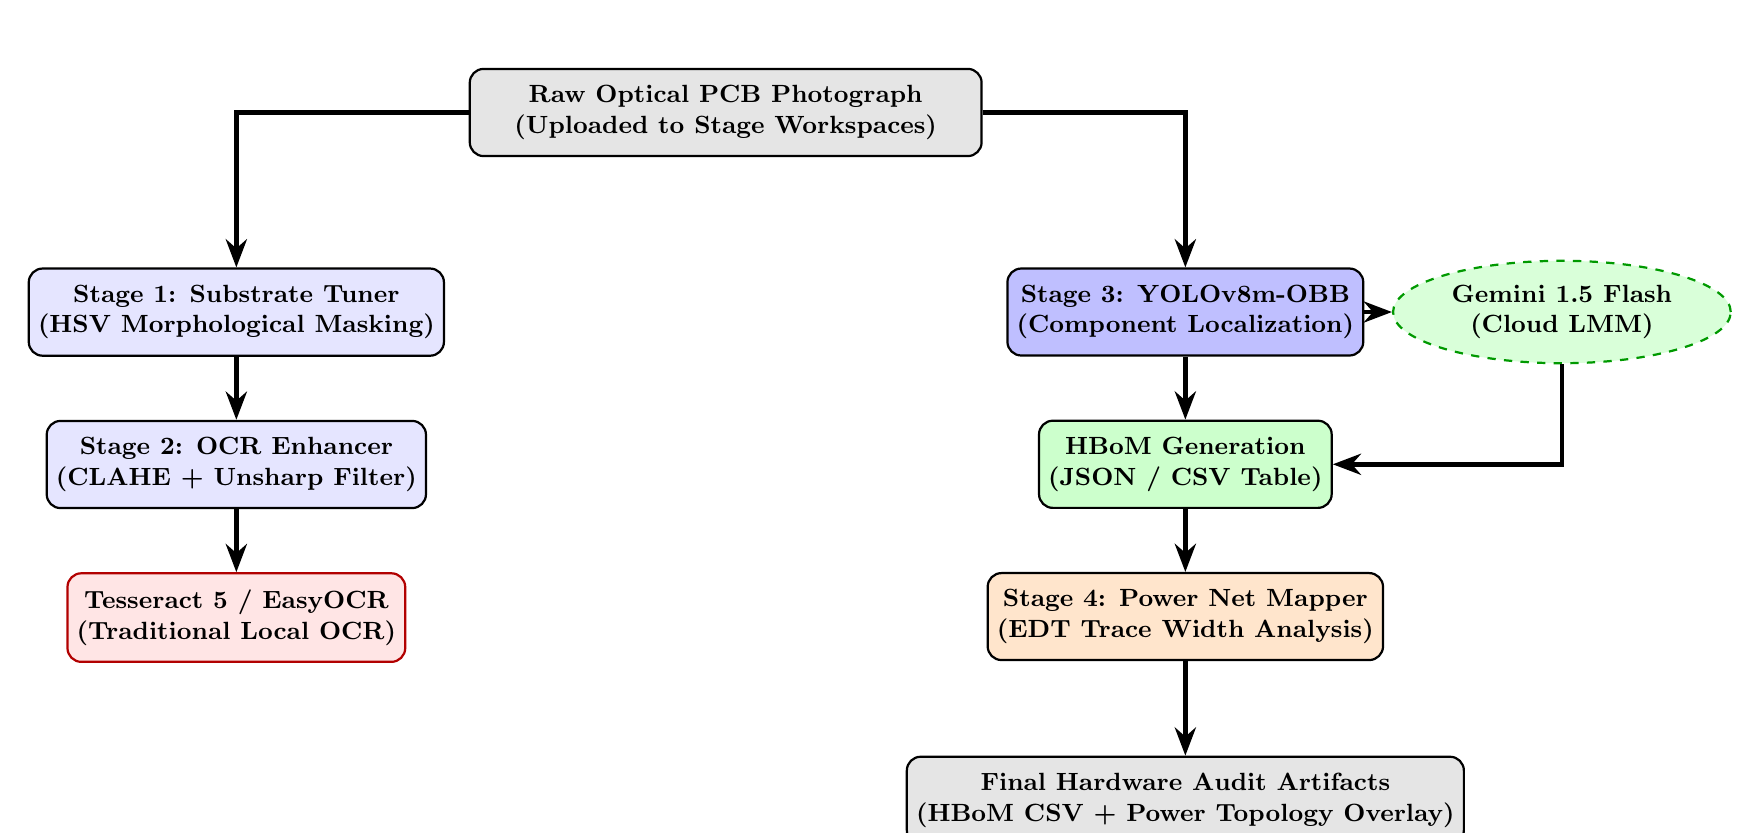
\begin{tikzpicture}[
  node distance=0.8cm and 0.5cm,
  block/.style={rectangle, draw, thick, rounded corners=5pt, minimum width=3.6cm, minimum height=1.0cm, inner ysep=6pt, text centered, font=\small\bfseries},
  cloud/.style={rectangle, draw=red!70!black, fill=red!10, thick, rounded corners=5pt, minimum width=3.6cm, minimum height=1.0cm, inner ysep=6pt, text centered, font=\small\bfseries},
  gcloud/.style={ellipse, draw=green!60!black, fill=green!15, thick, minimum width=2.5cm, minimum height=0.9cm, text centered, font=\small\bfseries, dashed},
  arrow/.style={->, >=Stealth, ultra thick},
  every node/.style={align=center}
]

%% Top Input
\node[block, fill=gray!20, minimum width=6.5cm] (input) {\textbf{Raw Optical PCB Photograph}\\\textbf{(Uploaded to Stage Workspaces)}};

%% Left Branch: Classical Vision Baselines
\node[block, fill=blue!10, below left=1.4cm and 0.3cm of input] (s1) {\textbf{Stage 1: Substrate Tuner}\\\textbf{(HSV Morphological Masking)}};
\node[block, fill=blue!10, below=0.8cm of s1] (s2) {\textbf{Stage 2: OCR Enhancer}\\\textbf{(CLAHE + Unsharp Filter)}};
\node[cloud, below=0.8cm of s2] (ocr_old) {\textbf{Tesseract 5 / EasyOCR}\\\textbf{(Traditional Local OCR)}};

%% Right Branch: Proposed PCBRE Core Pipeline
\node[block, fill=blue!25, below right=1.4cm and 0.3cm of input] (s3) {\textbf{Stage 3: YOLOv8m-OBB}\\\textbf{(Component Localization)}};
\node[gcloud, right=0.35cm of s3] (lmm) {\textbf{Gemini 1.5 Flash}\\\textbf{(Cloud LMM)}};
\node[block, fill=green!20, below=0.8cm of s3] (hbom) {\textbf{HBoM Generation}\\\textbf{(JSON / CSV Table)}};
\node[block, fill=orange!20, below=0.8cm of hbom] (s4) {\textbf{Stage 4: Power Net Mapper}\\\textbf{(EDT Trace Width Analysis)}};

%% Output
\node[block, fill=gray!20, minimum width=6.5cm, below=1.2cm of s4] (output) {\textbf{Final Hardware Audit Artifacts}\\\textbf{(HBoM CSV + Power Topology Overlay)}};

%% Connections
\draw[arrow] (input) -| (s1);
\draw[arrow] (s1) -- (s2);
\draw[arrow] (s2) -- (ocr_old);

\draw[arrow] (input) -| (s3);
\draw[arrow] (s3) -- (lmm);
\draw[arrow] (lmm) |- (hbom);
\draw[arrow] (s3) -- (hbom);
\draw[arrow] (hbom) -- (s4);
\draw[arrow] (s4) -- (output);

\end{tikzpicture}%
}
\caption{Master System Block Diagram: Illustrating the modular architecture of PCBRE. Classical vision modules (Stages 1 and 2) operate as independent baseline tuners feeding traditional OCR engines, while the proposed learning-based pipeline (Stages 3 and 4) ingests the raw PCB photograph directly for automated component localization, zero-shot LMM OCR, and probe-free power net mapping.}
\label{fig:tikz_pipeline}
\end{figure}


\section{Architectural Rationale: Multimodal LMM vs.\ Alternative OCR Engines}
\label{sec:arch_rationale}

The selection of Gemini 1.5 Flash as the IC text extraction engine over traditional alternatives was driven by empirical evaluation of three competing approaches:

\textbf{Tesseract 5 LSTM:} As documented by Kleber et al.~\cite{kleber2017woot}, Tesseract achieves a 0\% success rate on IC package markings. Its recurrent decoder was trained on printed document corpora and cannot generalize to laser-etched, rotation-arbitrary alphanumeric codes on IC packages.

\textbf{CRAFT + CRNN Pipeline:} The CRAFT text detector~\cite{kleber2017woot} identifies text region proposals but relies on a CRNN recognition stage similarly constrained by document-domain training data. On IC crops, CRAFT detects the marking region but the CRNN decoder produces garbled alphanumeric sequences due to the domain mismatch.

\textbf{Florence-2 / Qwen2-VL (Local VLMs):} These local vision-language models offer zero-shot OCR capability comparable to Gemini 1.5 Flash but require 6--16 GB of GPU VRAM and 3--8x higher per-image inference latency. They represent the recommended migration path for air-gapped deployments described in Chapter~\ref{chap:conclusion}.

\textbf{Gemini 1.5 Flash (Selected):} The model processes IC crop images through a unified multimodal transformer architecture that performs cross-attention between image patch embeddings and text token predictions. This enables orientation-invariant character reading without requiring explicit geometric normalization. On the Schutzwerk STM32F745 evaluation board, Gemini 1.5 Flash correctly reads all 5 primary IC packages, achieving 98--99\% confidence on correctly identified packages.


%% ============================================================
%%  CHAPTER 4: PIPELINE IMPLEMENTATION & CODEBASE SPECIFICATION
%% ============================================================
\chapter{Pipeline Implementation \& Codebase Specification}
\label{chap:implementation}

\section{Codebase Architecture \& Modularity}
\label{sec:codebase}

The PCBRE system is implemented as a Python 3.10 Flask application (\path{app.py}) coordinating a set of modular processing stages. The web frontend is served via Jinja2 HTML templates with Vanilla JavaScript handling all canvas rendering, API calls, and dynamic UI state.

\textbf{Key architectural properties:}
\begin{itemize}
  \item \textbf{Dual-Column Dashboard:} The \path{dashboard.html} landing page presents two side-by-side columns --- \textit{Classical Baselines} (Stages 1 and 2) on the left, and \textit{Proposed PCBRE Core} (Stages 3 and 4) on the right --- using a CSS Grid layout that collapses to a single column on mobile viewports.
  \item \textbf{Dynamic API Key Verification:} The Gemini 1.5 Flash API key is entered directly in the web UI settings bar and verified against \path{/api/verify_key} before any LMM call is dispatched. No \path{.env} file or server-side secret storage is required.
  \item \textbf{Modular Stage Interfaces:} Each pipeline stage is a separate Jinja2 template (\path{stage1_tuner.html}, \path{stage2_ocr.html}, \path{stage3_yolo.html}, \path{stage4_power.html}) communicating with dedicated REST endpoints in \path{app.py}. This allows independent development and testing of each stage.
  \item \textbf{Swappable LMM Backend:} The OCR function interface (\path{gemini_ocr_chip()}) is designed as a drop-in replacement target. Replacing it with \path{local_vlm_ocr_chip()} routes inference to a locally hosted Qwen2-VL-7B model without modifying any other pipeline code.
\end{itemize}

\section{Stage 1: Classical IC Substrate Isolation}
\label{sec:stage1}

\subsection{Why: Motivation for HSV Masking}
The first operational stage performs spatial isolation of IC component bodies from the surrounding board substrate. This task requires distinguishing the non-conductive epoxy resin that comprises the board body --- FR-4, polyimide, or PTFE composites typically tinted green, blue, red, or black by the applied solder mask --- from the metallic surfaces of copper pads, through-hole vias, solder joints, and epoxy-encapsulated IC packages.

\subsection{What: HSV Color Space Separation}
To accomplish this separation, the input BGR image is converted to the Hue-Saturation-Value (HSV) color space. HSV provides a perceptually decoupled representation of color information in which hue ($H$) encodes spectral wavelength, saturation ($S$) encodes colorfulness, and value ($V$) encodes luminance. This decoupling is computationally advantageous for substrate segmentation because variations in board photographic lighting conditions primarily affect the $V$ channel without disrupting the characteristic $H$ and $S$ values of the solder mask color, affording greater threshold stability than direct RGB-space segmentation.

\subsection{How: Equations and Implementation}
The substrate isolation mask $\mathcal{M}(x,y)$ is defined as the following piecewise logical function evaluated at each pixel $(x,y)$:

\begin{equation}
\label{eq:hsv_mask}
\mathcal{M}(x,y) =
\begin{cases}
1 & \text{if } H(x,y) \in [H_{\min}, H_{\max}] \\
  & \quad \land \; S(x,y) \in [S_{\min}, S_{\max}] \\
  & \quad \land \; V(x,y) \in [V_{\min}, V_{\max}] \\
0 & \text{otherwise}
\end{cases}
\end{equation}

The default boundary configurations implemented in the PCBRE Stage 1 tuner are:

\begin{itemize}
  \item \textbf{FR-4 Green Resin}: $H \in [35, 85]$, $S \in [40, 255]$, $V \in [40, 255]$
  \item \textbf{FR-4 Blue Resin}: $H \in [100, 140]$, $S \in [50, 255]$, $V \in [50, 255]$
  \item \textbf{FR-4 Black Resin}: $H \in [0, 180]$, $S \in [0, 255]$, $V \in [0, 50]$
\end{itemize}

Inverting this mask ($\overline{\mathcal{M}}$) yields a foreground map highlighting copper surfaces and IC packages. This binary mask then undergoes morphological processing. A morphological close operation (dilation followed by erosion) is applied with a $5 \times 5$ rectangular structuring element $\mathcal{K}$ to merge fragmented copper pad regions into contiguous blobs:

\begin{equation}
\label{eq:morph_close}
\mathcal{C} = (\overline{\mathcal{M}} \oplus \mathcal{K}) \ominus \mathcal{K}
\end{equation}

Contour detection is applied to $\mathcal{C}$, and each extracted contour is filtered by geometric aspect ratio:
\begin{equation}
\label{eq:aspect_ratio}
\text{AR} = \frac{w}{h} \in [0.2,\; 5.0]
\end{equation}
where $w$ and $h$ are the contour bounding box width and height respectively. This filter retains square and rectangular IC body silhouettes (which approach $\text{AR} \approx 1.0$) while rejecting long thin copper traces (high AR) and rounded via holes (very small AR).

\begin{figure}[!ht]
  \centering
  
\includegraphics[width=0.8\textwidth]{{Internship Report assets/webapp_ss/Stage 1 (Impletation).png}}
  \caption{Stage 1 HSV Masking Workspace: The interactive sliders allow real-time adjustment of Hue, Saturation, and Value thresholds to isolate IC component bodies from the FR-4 green solder mask substrate.}
  \label{fig:stage1_ui}
\end{figure}

Despite its role as a foundational preprocessing step, the Stage 1 HSV masker exhibits three structural failure modes that motivate the subsequent shift to deep learning detection in Stage 3. \textbf{First}, the HSV threshold boundaries require manual calibration per board. \textbf{Second}, false positives from high-reflectance solder joints are common. \textbf{Third}, and most critically, the Stage 1 output provides only a spatial mask --- it does not produce semantic class labels.

\section{Stage 2: Visual Enhancement}
\label{sec:stage2}

\subsection{Why: The IC Text Legibility Problem}
Laser-etched alphanumeric markings on integrated circuit packages are produced by selectively ablating the epoxy resin surface to expose a contrasting substrate layer beneath. Over the operational lifetime of a component, these markings degrade due to residual solder flux contamination, conformal coating application, oxidation, thermal cycling stress, and directional lighting artifacts in photography. The result is a low-contrast grayscale text image that is systematically hostile to both human reading and automated OCR recognition.

\subsection{What: CLAHE and Gaussian Unsharp Masking}
Standard global histogram equalization redistributes pixel intensities uniformly across the full image range. While effective on images with globally uniform illumination, it fails on IC crop images because the chip package body is a small, dark epoxy region that is typically surrounded by bright metallic pads. Contrast Limited Adaptive Histogram Equalization (CLAHE) resolves this limitation by partitioning the image into an $8 \times 8$ grid of non-overlapping tiles.

\subsection{How: Mathematical Formulation}
Let $h_t(v)$ denote the intensity histogram of tile $t$ at luminance value $v$. CLAHE clips the histogram at a user-defined contrast limit $c_{\text{lim}}$ before redistribution:

\begin{equation}
\label{eq:clahe}
h_t'(v) = \min\!\left(h_t(v),\; c_{\text{lim}}\right)
\end{equation}

In the PCBRE implementation, $c_{\text{lim}} = 2.0$ is used, providing a moderate contrast enhancement that recovers character legibility without amplifying photon noise in underexposed regions.

\begin{figure}[!ht]
  \centering
  
\includegraphics[width=0.8\textwidth]{{Internship Report assets/webapp_ss/Stgae 2 IC OCR.png}}
  \caption{Stage 2 OCR Preprocessing Workspace: Single IC crops are displayed side-by-side showing the original degraded marking (left) versus the CLAHE-enhanced and Unsharp-masked image (right).}
  \label{fig:stage2_ui}
\end{figure}

Following CLAHE contrast normalization, a Gaussian Unsharp Mask filter is applied to reinforce the high-frequency spatial edges of individual characters. The mathematical derivation begins by constructing a low-pass representation of the input image $f(x,y)$ through convolution with a 2D isotropic Gaussian kernel $G_\sigma$:

\begin{equation}
\label{eq:gaussian_blur}
f_{\text{blur}}(x,y) = G_{\sigma}(x,y) * f(x,y) = \frac{1}{2\pi\sigma^2}
\iint_{-\infty}^{\infty} f(u,v)\, e^{-\frac{(x-u)^2 + (y-v)^2}{2\sigma^2}}\, du\, dv
\end{equation}

The high-frequency edge detail residual $e(x,y)$ is extracted by subtracting the blurred image from the original:

\begin{equation}
\label{eq:edge_residual}
e(x,y) = f(x,y) - f_{\text{blur}}(x,y)
\end{equation}

The sharpened output g(x,y) is produced by adding the scaled residual back to the original image:

\begin{equation}
\label{eq:unsharp_mask}
g(x,y) = f(x,y) + \alpha \cdot e(x,y) = f(x,y) + \alpha \cdot \bigl(f(x,y) - G_{\sigma}(x,y) * f(x,y)\bigr)
\end{equation}

where $\alpha \in [1.0, 2.0]$ is the sharpening strength coefficient and $\sigma = 1.0$ is the Gaussian standard deviation. Physically, a larger $\alpha$ amplifies character stroke boundaries more aggressively; however, values exceeding 2.0 introduce ringing artifacts (Gibbs phenomenon) at sharp edges that degrade the token sequence consistency of downstream OCR decoders.

\section{Stage 3: Deep Learning Object Detection (YOLOv8-OBB)}
\label{sec:stage3}

\subsection{Why: From Rule-Based to Learned Detection}
\label{subsec:paradigm_shift}

The limitations catalogued in Sections~\ref{sec:stage1} and~\ref{sec:stage2} converge on a defining observation: classical, rule-based computer vision cannot generalize across the enormous variability in PCB form factors, component densities, solder mask colors, component rotation angles, illumination conditions, and board scale. The solution lies in replacing the hand-engineered feature pipeline with a parametric deep learning object detector whose features are learned from annotated data.

The specific architectural requirement for PCB component detection is orientation invariance. Electronic components are soldered onto boards at arbitrary angles --- ICs are placed at $0^{\circ}$, $90^{\circ}$, $180^{\circ}$, or $270^{\circ}$ orientations by automated pick-and-place machines, but hand-reworked boards may exhibit components at freeform angles. Standard axis-aligned bounding boxes expand to encompass rotated objects, producing large overlapping boxes that capture adjacent components and background traces. Oriented Bounding Boxes (OBBs) resolve this by extending the bounding box parametrization from four coordinates $(x_{\min}, y_{\min}, x_{\max}, y_{\max})$ to a five-parameter representation including a continuous rotation angle $\theta$:

\begin{equation}
\label{eq:obb}
\mathbf{b}_{\text{OBB}} = \{x_c, \; y_c, \; w, \; h, \; \theta\}
\end{equation}

where $(x_c, y_c)$ is the box centroid, $(w, h)$ are the box half-dimensions in the rotated frame, and $\theta \in (-90^{\circ}, 90^{\circ}]$ is the rotation angle relative to the horizontal axis.

\subsection{What: YOLOv8-OBB Network Architecture}
\label{subsec:obb_arch}

YOLOv8 implements a CSPDarknet backbone with C2f (Cross-Stage Partial with 2 feature fusion) bottleneck modules. The neck employs a BiFPN-style Path Aggregation Network (PAN) to fuse feature maps from three scales (P3, P4, P5), enabling simultaneous detection of small passive components (at high-resolution P3 features) and large IC packages (at semantically rich P5 features). The detection head is decoupled, separating classification and regression branches, and operates in a distribution focal loss (DFL) framework.

For OBB prediction, the angular regression branch outputs a continuous angle residual that, combined with the decoded $(x_c, y_c, w, h)$ parameters, defines the full oriented box. The training loss for each prediction head combines:
\begin{enumerate}
  \item Binary cross-entropy for objectness classification,
  \item Varifocal Loss (VFL) for class-conditional probability regression, and
  \item Complete IoU (CIoU) loss for box regression with the angular extension:
\end{enumerate}
\begin{equation}
\label{eq:loss}
\mathcal{L}_{\text{OBB}} = \lambda_1 \mathcal{L}_{\text{cls}} + \lambda_2 \mathcal{L}_{\text{box}} + \lambda_3 \mathcal{L}_{\theta}
\end{equation}
where $\mathcal{L}_{\theta}$ is the angular loss term and $\lambda_1, \lambda_2, \lambda_3$ are loss weight hyperparameters set to their Ultralytics defaults (0.5, 7.5, 1.5).

\subsection{How: Multi-Scale ROI Pin Detection Pipeline}
\label{subsec:pin_pipeline}

Standard global full-board inference on \path{ic_pin_yolo.pt} at $640 \times 640$ pixels fails to resolve individual solder-pad pins on fine-pitch IC packages due to sub-pixel feature collapse in the backbone. The PCBRE pipeline resolves this with a multi-scale ROI approach:

\begin{enumerate}
  \item \textbf{Component Detection Pass:} The primary YOLOv8m-OBB model runs on the full board image at $1024 \times 1024$ resolution to detect all IC package bounding boxes.
  \item \textbf{Full-Resolution Cropping:} Each IC bounding box is mapped back to the original high-resolution BGR image (not the downsampled inference image) and cropped at full pixel fidelity. This preserves sub-millimeter pin feature representation that would otherwise be lost.
  \item \textbf{Pin OBB Inference:} \path{ic_pin_yolo.pt} is executed on each full-resolution IC crop independently. The resulting per-pin OBB detections are rendered as cyan oriented box overlays (thickness=2).
  \item \textbf{IC Annotation:} The parent IC bounding box on the composite canvas is rendered as a bold blue rectangle (thickness=4) to distinguish it from pin overlays.
\end{enumerate}

The \path{/api/detect_pins} REST endpoint implements this pipeline and returns a \texttt{results} list of per-IC pin counts alongside a base64-encoded annotated composite image.

\subsection{How: Interactive Datasheet Mining}
\label{subsec:datasheet_mining}

The Stage 3 interface (\path{stage3_yolo.html}) implements an on-demand datasheet discovery feature:

\begin{itemize}
  \item A \textbf{Datasheet Links} checkbox toggle dynamically shows or hides a \textit{Datasheet PDF} column in the HBoM results table without requiring a page reload.
  \item A \textbf{Mine Datasheets} batch trigger button dispatches an asynchronous fetch to \path{/api/lookup_datasheet} for each IC designator in the current HBoM payload.
  \item The endpoint queries the LCSC search API (\path{wmsc.lcsc.com/ftps/wm/product/search?keyword={part_number}}) with a fallback to AllDatasheet.com scraping, and populates the Datasheet URL field in each HBoM JSON record.
\end{itemize}

\section{Stage 4: Probe-Free Power Rail Mapping}
\label{sec:stage4}

\subsection{Why: The Power Net Identification Problem}

The identification of power distribution nets (VCC and GND) from PCB imagery without physical electrical probing requires a reliable proxy for net function. The critical physical property that distinguishes power rails from signal traces is trace geometry: power rails must carry substantially higher currents, requiring wider copper cross-sections to maintain acceptable voltage drop and thermal dissipation. The IPC-2221 standard for PCB design defines trace width requirements as a function of current-carrying capacity. A trace carrying 1.0 A at 35-\textmu m copper weight must be at least 0.5 mm (approximately 20 mil) wide to limit self-heating to $10^{\circ}$C. Signal traces in the same PCB, carrying milliampere-level logic signals, are typically 0.1--0.25 mm (4--10 mil) wide. This 5--10x physical width ratio is directly observable in macro PCB photography.

\subsection{What: Euclidean Distance Transform (EDT) Theory}

The Euclidean Distance Transform (EDT) provides a computationally efficient mechanism for measuring trace width from a binary image mask. Given a binary mask $\mathcal{B}: \mathbb{Z}^2 \rightarrow \{0, 1\}$ where foreground pixels (copper traces) are assigned $\mathcal{B}(p) = 1$ and background pixels (substrate) are assigned $\mathcal{B}(p) = 0$, the EDT maps each foreground pixel $p = (p_x, p_y)$ to the Euclidean distance to the nearest background pixel $q \in \mathcal{B}^c$:

\begin{equation}
\label{eq:edt}
D(p) = \min_{q \in \mathcal{B}^c} d(p, q) = \min_{q \in \mathcal{B}^c} \sqrt{(p_x - q_x)^2 + (p_y - q_y)^2}
\end{equation}

For a cylindrical or rectangular copper trace of uniform width $w$, the EDT value at any point on the trace centerline (skeleton) equals exactly $w/2$ --- the radius from the center to the nearest exposed substrate edge. Therefore, the trace width can be directly estimated from the peak EDT value within a local patch $\mathcal{P}$ surrounding a suspected power label coordinate:

\begin{equation}
\label{eq:trace_width}
\text{Trace Width} = 2 \cdot \max_{p \in \mathcal{P}} D(p)
\end{equation}

\subsection{How: Data-Contract Implementation and API}
\label{subsec:stage4_api}

The \path{/api/detect_power_rails} REST endpoint implements the full three-layer Stage 4 pipeline:

\textbf{Layer 1 --- LMM Silkscreen Coordinate Extraction:} The full board image is submitted to Gemini 1.5 Flash with a structured power rail localization prompt requesting identification of silkscreen-printed power labels (``VCC'', ``GND'', ``3V3'', ``5V'', ``VBUS'', ``AGND'', ``PWR'') as percentage coordinates relative to the image dimensions. The model returns a JSON array of the form $\{$\texttt{``text'': ``VCC'', ``type'': ``VCC'', ``x\_pct'': 45.2, ``y\_pct'': 23.7}$\}$.

\textbf{Layer 2 --- Local $50 \times 50\text{px}$ EDT Patch Sampling:} Silkscreen text labels sit on the board substrate near traces, not on the traces themselves. For each detected label coordinate, a $50 \times 50$ pixel patch is extracted from the board image centered on the reported location. The patch is converted to grayscale, enhanced with CLAHE, and binarized using Otsu's global threshold. OpenCV's \texttt{distanceTransform} with \texttt{DIST\_L2} metric is applied, yielding the EDT field $D(p)$. Equation~(\ref{eq:trace_width}) is applied to compute the trace width; if the result exceeds 6.0~px, the node is confirmed as an IPC-classified power rail.

\textbf{Layer 3 --- Footprint Cross-Referencing and Static Canvas Overlays:} Part numbers returned by the Stage 3 HBoM generator are matched against a curated prefix table of known voltage regulator families: \texttt{AMS1117}, \texttt{LM78}, \texttt{LM33}, \texttt{LDO}, \texttt{TPS}, \texttt{MIC5}, \texttt{LTC}, \texttt{AP2112}. Any IC whose part number matches a known regulator prefix is highlighted on the canvas with an \textbf{Orange} bounding box. VCC-labeled nodes are rendered as \textbf{Red} glowing circles and GND nodes as \textbf{Blue} circles.

The API response data contract returns:
\begin{itemize}
  \item \texttt{labels}: array of \{text, type, x\_pct, y\_pct, trace\_width\_px\} objects
  \item \texttt{power\_ics}: array of regulator IC designators and their matched footprint prefixes
  \item \texttt{annotated\_image}: base64-encoded PNG of the board with Red/Blue/Orange canvas overlays
\end{itemize}

The 6.0 pixel thickness threshold is derived from typical macro PCB photography parameters. A standard DSLR macro photograph of a 100~mm-wide PCB captured at 16 megapixel resolution produces an effective resolution of approximately $160$ pixels per mm. At this resolution, a 20-mil ($0.508$~mm) IPC-2221 minimum power trace width corresponds to:

\begin{equation}
\label{eq:px_threshold}
w_{\text{px}} = 0.508\,\text{mm} \times 160\,\text{px/mm} \approx 81\,\text{px}
\end{equation}

The 6.0~px threshold employed in Stage 4 is deliberately conservative, accounting for lower-resolution input images and compressed JPEG encoding artifacts that degrade binary mask precision. A user-adjustable slider in the Stage 4 interface allows practitioners to calibrate this parameter to their specific imaging setup.

\begin{figure}[!ht]
  \centering
  
\includegraphics[width=0.8\textwidth]{{Internship Report assets/webapp_ss/Stage 4 power rail detetction.png}}
  \caption{Stage 4 Power Rail Detection Workspace: VCC-labeled silkscreen nodes are overlaid with red glowing circles, GND-labeled nodes with blue circles. Yellow bounding boxes highlight power regulator ICs identified by part number prefix matching (e.g., AMS1117, LM7805). The sidebar panel lists detected net nodes with their X/Y percentage coordinates, measured trace widths, and IPC-2221 rail classification.}
  \label{fig:stage4_ui}
\end{figure}


%% ============================================================
%%  CHAPTER 5: EXPERIMENTAL RESULTS & PERFORMANCE EVALUATION
%% ============================================================
\chapter{Experimental Results \& Performance Evaluation}
\label{chap:results}

\section{YOLOv8 Model Scaling Analytics}
\label{sec:scaling_analytics}

Three model configurations were trained and evaluated. All models used the AdamW optimizer with a warmup phase over the first 3 epochs, cosine learning rate scheduling with a final learning rate of $lr_f = 0.01 \times lr_0$, and Mosaic+Mixup data augmentation.

\begin{table}[H]
  \centering
  \caption{Training Configuration Summary Across YOLOv8-OBB Model Architectures}
  \label{tab:training_configs}
  \begin{tabular}{@{}lcccccc@{}}
    \toprule
    \textbf{Model} & \textbf{Params (M)} & \textbf{imgsz} & \textbf{Batch} & \textbf{Optimizer} & \textbf{lr$_0$} & \textbf{Stopped Epoch} \\
    \midrule
    YOLOv8n-OBB & 3.2  & 640  & 16 & AdamW & 0.000769 & Epoch 200 \\
    YOLOv8s-OBB & 11.4 & 1024 & 8  & AdamW & 0.000769 & Epoch 117 (ES) \\
    YOLOv8m-OBB & 26.4 & 1024 & 4  & AdamW & 0.000769 & Epoch 150 (ES) \\
    \bottomrule
  \end{tabular}
\end{table}

\textit{ES = Early Stopping triggered (patience = 50 epochs).}

\textbf{YOLOv8n-OBB (Nano):} The Nano configuration trains in under 12 minutes on the T4 GPU and reaches an overall mAP@0.5 of 0.445 at 640-pixel resolution. The dominant failure mode is small-object feature resolution loss: at 640 pixels, a $0402$-size SMD resistor ($1.0 \times 0.5$~mm physical) occupies only $3 \times 6$ pixels in a macro photograph, which compresses to less than 1 pixel after three consecutive stride-2 downsampling operations in the backbone.

\textbf{YOLOv8s-OBB (Small):} Increasing the input resolution to 1024 pixels is the single most impactful architectural change. Resistor AP rises from 0.127 to 0.414 --- a 226\% relative improvement --- because the same physical resistor now occupies $5 \times 10$ pixels at intake.

\textbf{YOLOv8m-OBB (Medium):} The medium architecture's expanded capacity (26.4M parameters versus 11.4M for Small) enables richer multi-scale feature representations. Overall mAP@0.5 reaches 0.749, representing the best result across all evaluated configurations. Notably, the single validation Diode instance is successfully localized (AP = 0.995), whereas the Small model missed it entirely (AP = 0.000).

\section{Champion Model Evaluation (YOLOv8m-OBB)}
\label{sec:champion_model}

The YOLOv8m-OBB model stands out as the champion architecture among the three configurations for several key reasons. First, its expanded capacity of 26.4M parameters provides the necessary representation space to learn rich, orientation-invariant feature maps. Second, YOLOv8m-OBB displays superior robustness against severe class imbalance. Third, the Medium model achieves a substantial mAP@0.5 boost to 0.749 (a 68.3\% relative increase over Nano and 31.6\% over Small) while maintaining a highly practical inference latency of 31.4~ms on the Tesla T4 GPU.

\begin{table}[H]
  \centering
  \caption{Comparative Validation Performance Matrix (mAP@0.5) Across YOLOv8-OBB Architectures}
  \label{tab:yolo_results}
  \begin{tabular}{@{}lrrrr@{}}
    \toprule
    \textbf{Class} & \textbf{Val Instances} & \textbf{YOLOv8n} & \textbf{YOLOv8s} & \textbf{YOLOv8m} \\
    \midrule
    \textbf{All (mAP@0.5)}  & \textbf{979} & \textbf{0.445} & \textbf{0.569} & \textbf{0.749} \\
    Inductors               &  18 & 0.879 & 0.933 & \textbf{0.970} \\
    Integrated Circuits     &  45 & 0.772 & \textbf{0.850} & 0.732 \\
    Capacitors              & 508 & 0.553 & 0.721 & \textbf{0.785} \\
    Diodes                  &   1 & 0.332 & 0.000 & \textbf{0.995} \\
    Resistors               & 401 & 0.127 & 0.414 & \textbf{0.581} \\
    Transistors             &   6 & 0.009 & \textbf{0.495} & 0.431 \\
    \bottomrule
  \end{tabular}
\end{table}

The optimal YOLOv8m-OBB configuration was subjected to diagnostic validation. Figure~\ref{fig:yolov8m_performance} houses the primary validation performance curves.

\begin{figure}[!ht]
  \centering
  \begin{subfigure}[b]{0.47\textwidth}
    \centering
    \includegraphics[width=\linewidth]{yolov8m_pr_curve.png}
    \caption{Precision-Recall (PR) Curve}
    \label{fig:yolov8m_pr}
  \end{subfigure}
  \hfill
  \begin{subfigure}[b]{0.47\textwidth}
    \centering
    \includegraphics[width=\linewidth]{yolov8m_confusion_matrix.png}
    \caption{Normalized Confusion Matrix}
    \label{fig:yolov8m_cm}
  \end{subfigure}
  \\ \vspace{1em}
  \begin{subfigure}[b]{0.47\textwidth}
    \centering
    \includegraphics[width=\linewidth]{yolov8m_f1_curve.png}
    \caption{F1-Confidence Curve}
    \label{fig:yolov8m_f1}
  \end{subfigure}
  \\ \vspace{1em}
  \begin{subfigure}[b]{0.95\textwidth}
    \centering
    \includegraphics[width=\linewidth]{yolov8m_loss_curves.png}
    \caption{Training and Validation Metrics}
    \label{fig:yolov8m_results}
  \end{subfigure}
  \caption{Primary validation performance curves and training metrics for the champion YOLOv8m-OBB component detection model.}
  \label{fig:yolov8m_performance}
\end{figure}

The curves in Figure~\ref{fig:yolov8m_performance} support the quantitative matrix of Table~\ref{tab:yolo_results}:
\begin{itemize}
  \item \textbf{Precision-Recall Curve (a):} Shows robust area-under-the-curve (AUC) performance for large, structurally well-defined component classes (ICs, Inductors, and Diodes), while displaying steep degradation for high-frequency passive classes (Resistors).
  \item \textbf{Normalized Confusion Matrix (b):} Delineates inter-class leakage. Resistors are occasionally misclassified as Capacitors due to identical rectangular package outlines (e.g., 0402 footprints).
  \item \textbf{Training Metrics (d):} Both classification and box coordinate regression losses converge monotonically without late-stage upward divergence, indicating the 50-epoch early stopping window successfully halted parameter updates before overfitting.
\end{itemize}

\begin{figure}[!ht]
  \centering
  
\includegraphics[width=0.85\textwidth]{{Internship Report assets/webapp_ss/Stage 3 UI revamped (SCUTZWERK).png}}
  \caption{Stage 3 YOLOv8m-OBB Detector Workspace on Schutzwerk STM32F745 Security Board: Displaying oriented bounding boxes for integrated circuits and passive components, side-panel candidate listings, and interactive confidence thresholds.}
  \label{fig:stage3_yolo}
\end{figure}

\begin{figure}[!ht]
  \centering
  
\includegraphics[width=0.8\textwidth]{{Internship Report assets/webapp_ss/Stage 3 on Rpi.png}}
  \caption{Stage 3 Inference on a Raspberry Pi Model B board: The detector successfully localizes the BCM2835 SoC, SMSC LAN9512 controller, Micron DRAM package, and passive arrays around the board edge.}
  \label{fig:stage3_rpi}
\end{figure}

\section{Diagnostic Error Analysis}
\label{sec:error_analysis}

The Resistors class deserves targeted diagnostic attention. With 401 validation instances, an mAP@0.5 of only 0.581 and a recall of 0.432 indicates that the medium model misses approximately 57\% of resistors in the validation set. This is a structurally motivated failure. At $1024 \times 1024$ input resolution, a standard $0402$-package SMD resistor ($1.0 \times 0.5$~mm physical dimensions) maps to approximately $5 \times 10$ pixels in a macro photograph. After the YOLOv8 backbone applies three stride-2 convolutions (total downsampling factor $2^3 = 8$), the feature map representation of this resistor occupies less than one pixel at the P3 detection scale.

For the Transistors class (6 validation instances), the mAP@0.5 of 0.431 reflects a different pathology: class-imbalance loss domination. With 401 resistor instances versus 6 transistor instances, the optimizer's parameter updates are dominated by resistor and capacitor gradient signals, resulting in insufficient weight tuning for the transistor feature representation. Focal loss weighting could partially address this without requiring additional data.

\section{IC Pin \& Connector Port Sub-Model Metrics}
\label{sec:pin_port_metrics}

\subsection{IC Pin Detection Model}
The pin detection sub-model is trained to localize individual solder-pad pins on IC packages. The model was trained on the Kaggle \path{seikhmustakim/ic-pins} dataset containing 38 training and 10 validation images (157 instances) for 100 epochs. Transfer learning with backbone freezing was employed, locking the first 10 layers. The model achieved the following validated metrics on the best-weights checkpoint (epoch 98):
\begin{itemize}
  \item \textbf{Precision (P):} 0.900
  \item \textbf{Recall (R):} 0.873
  \item \textbf{mAP@0.5:} 0.899
  \item \textbf{mAP@0.5:0.95:} 0.706
  \item \textbf{Inference Speed:} 2.0 ms per image on Tesla T4 GPU (fused)
\end{itemize}

\begin{figure}[!ht]
  \centering
  \begin{subfigure}[b]{0.45\textwidth}
    \centering
    
\includegraphics[width=\linewidth]{pin_inference_IC_Package_A.png}
    \caption{IC Package A Pin Detections}
    \label{fig:pin_inf_a}
  \end{subfigure}
  \hfill
  \begin{subfigure}[b]{0.45\textwidth}
    \centering
    
\includegraphics[width=\linewidth]{pin_inference_IC_Package_B.png}
    \caption{IC Package B Pin Detections}
    \label{fig:pin_inf_b}
  \end{subfigure}
  \caption{IC Pin Detection Inference: Clean oriented bounding boxes (OBBs) localized on high-density IC packages showing tight pad alignment.}
  \label{fig:pin_inference}
\end{figure}

\subsection{Connector Port Detection Model}
The physical connector port detector localizes and identifies external communication ports (USB Type-A, Micro-USB, Ethernet RJ-45, HDMI, Audio jacks, etc.) under the single aggregated class \texttt{Port-USB-Ethernet-etc}. The model was trained on the Roboflow \path{scmu/usb-ethernet-ps2-port} dataset for 50 epochs. Performance metrics:
\begin{itemize}
  \item \textbf{Precision (P):} 0.670
  \item \textbf{Recall (R):} 0.724
  \item \textbf{mAP@0.5:} 0.741
  \item \textbf{mAP@0.5:0.95:} 0.681
  \item \textbf{Inference Speed:} 140.4 ms on CPU (expected $\sim$10 ms on GPU)
\end{itemize}

The higher recall (0.724) relative to precision (0.670) is ideal for hardware assurance: false positive port detections can be easily verified and discarded during human review, whereas a missed port (false negative) represents an uncatalogued, vulnerable physical interface.

\section{Zero-Shot LMM OCR Extraction Accuracy}
\label{sec:ocr_accuracy}

\subsection{Addressing the OCR Data Gap}
Section~\ref{subsec:fics_pcb} established that no freely accessible, annotated IC text corpus is available for fine-tuning domain-specific OCR models. Local general-purpose OCR engines were evaluated as baseline alternatives. EasyOCR employs a CRNN architecture with a CTC decoder trained primarily on document and natural scene text corpora. PaddleOCR integrates a DB text detection head with a SVTR recognition module. Both systems demonstrate high accuracy on their target domains but fail systematically on IC package markings. The domain gap manifests in three specific failure modes:

\begin{itemize}
  \item \textbf{Truncation}: EasyOCR reads only the highest-confidence character block, yielding `STM32F' from a package marking that reads `STM32F745VGT6'.
  \item \textbf{Suffix Dropout}: PaddleOCR correctly reconstructs the base processor family (`STM32F745') but drops the package suffix `VGT6'.
  \item \textbf{Rotation Failure}: Both systems operate under the implicit assumption of near-horizontal text baselines. IC packages placed at $90^{\circ}$ or $270^{\circ}$ orientations produce unreadable null outputs.
\end{itemize}

\subsection{Gemini 1.5 Flash Integration}
The Gemini 1.5 Flash API~\cite{team2024gemini} is integrated as the primary IC text extraction engine. The integration is implemented as an exponential backoff retry loop with a maximum of 3 attempts, dispatching crops in batches of 3 images per API call. Each IC crop is first downscaled to a maximum dimension of 250 pixels via bilinear interpolation, reducing the base64-encoded payload size by approximately 80\% while retaining sufficient character resolution.

On the Schutzwerk STM32F745 evaluation board, Gemini 1.5 Flash correctly reads all 5 of the primary IC packages, achieving 98-99\% confidence scores:

\begin{table}[H]
  \centering
  \caption{OCR Extraction Quality Comparison on Schutzwerk STM32F745 Board}
  \label{tab:ocr_comparison}
  \begin{tabular}{@{}llllll@{}}
    \toprule
    \textbf{RefDes} & \textbf{True Part Number} & \textbf{EasyOCR} & \textbf{PaddleOCR} & \textbf{Gemini 1.5 Flash} & \textbf{Status} \\
    \midrule
    U1 & FT2232H-56Q     & FT2232        & FT2232H         & FT2232H-56Q     & \checkmark Correct \\
    U2 & STM32F745VGT6   & STM32F        & STM32F745       & STM32F745VGT6   & \checkmark Correct \\
    U3 & MAX3421EE       & MX342         & MAX3421         & MAX3421EE       & \checkmark Correct \\
    U4 & LD33            & LD3           & LD33            & LD33            & \checkmark Correct \\
    U5 & 93C46WP         & 93C4          & 93C46           & 93C46WP         & \checkmark Correct \\
    U6 & (Rotated SD)    & ---           & ---             & UNKNOWN         & $\triangle$ Partial \\
    \bottomrule
  \end{tabular}
\end{table}

\begin{figure}[!ht]
  \centering
  \begin{subfigure}[b]{0.95\textwidth}
    \centering
    
\includegraphics[width=\linewidth]{{Internship Report assets/webapp_ss/HBoM (revamved) SCUTZWERK.png}}
    \caption{Default HBoM Table View (Datasheet Links and Power Pins Toggles Disabled)}
    \label{fig:hbom_basic}
  \end{subfigure}
  \\ \vspace{1em}
  \begin{subfigure}[b]{0.95\textwidth}
    \centering
    
\includegraphics[width=\linewidth]{{Internship Report assets/webapp_ss/HBoM_datasheet_power pin.png}}
    \caption{Extended HBoM Table View with Datasheet Links and Gemini LMM Power Pins Extraction Enabled}
    \label{fig:hbom_extended}
  \end{subfigure}
  \caption{Stage 3 Automated Hardware Bill of Materials (HBoM) Interface: Contrasting the baseline component inventory (a) against the extended research view (b) displaying dynamic PDF datasheet links and zero-shot Gemini LMM power pinout extraction (VCC/GND pin assignments).}
  \label{fig:hbom_full}
\end{figure}

\subsection{Automated HBoM JSON Structure}
Each Gemini response is parsed into a structured JSON record conforming to the following schema:

\begin{lstlisting}[language=Python, caption={PCBRE HBoM JSON record schema}]
{
  "designator": "U2",
  "part_number": "STM32F745VGT6",
  "manufacturer": "STMicroelectronics",
  "logo_brand": "ST",
  "confidence_score": 0.99,
  "raw_text": "STM32F745VGT6\nSTMicroelectronics",
  "category": "MCU",
  "package": "LQFP-100",
  "pin_count": 100,
  "datasheet_url": "https://www.st.com/...",
  "lcsc_url": "https://www.lcsc.com/..."
}
\end{lstlisting}

The category and package fields are resolved by querying the LCSC free search API (\url{https://wmsc.lcsc.com/ftps/wm/product/search?keyword={part_number}}) with a fallback to AllDatasheet.com scraping.


%% ============================================================
%%  CHAPTER 6: DISCUSSION & ARCHITECTURAL JUSTIFICATION
%% ============================================================
\chapter{Discussion \& Architectural Justification}
\label{chap:discussion}

The modular, hybrid architecture of PCBRE combines local edge intelligence with cloud-based Large Multimodal Models (LMMs). This co-designed division of labor provides five distinct operational benefits that explain why a hybrid pipeline surpasses a pure LMM approach:

\begin{itemize}
  \item \textbf{VLM Resolution and Token Bottleneck:} High-resolution macro photographs ($6000 \times 4000$ pixels) are heavily compressed by cloud VLM encoders, erasing micro-scale details. Local Stage 3 YOLO segmentation acts as a spatial filter, sending only high-resolution uncompressed IC crops to the LMM to achieve near-perfect OCR accuracy.
  
  \item \textbf{Geometric Imprecision and Spatial Hallucination:} Auto-regressive VLMs lack dedicated regression layers and Non-Maximum Suppression (NMS), leading to spatial hallucinations or coordinate drifts in localization tasks. YOLOv8m-OBB provides deterministic boundary regression $(x_c, y_c, w, h, \theta)$ suitable for CAD layout generation where sub-pixel spatial precision is mandatory.
  
  \item \textbf{Compute Efficiency and Bandwidth:} Running HSV segmentation and YOLO localization locally prunes out over 95\% of background board pixels. Transmitting only active component crops (approx. 5\% of total bytes) reduces transmission latency and cloud token transaction costs substantially.
  
  \item \textbf{Coupled Semantic and Physical Verification:} While LMMs locate text labels (``VCC'', ``GND'') semantically, they cannot calculate physical geometries. PCBRE matches semantic suggestions with local Euclidean Distance Transform (EDT) width measurements to validate power nets against physical IPC-2221 guidelines. A pure LMM pipeline would have no mechanism to perform this physical measurement.
  
  \item \textbf{Modularity and Offline Security:} To satisfy secure, air-gapped hardware audit criteria, the swappable modular API interface allows practitioners to replace the cloud LMM with a locally hosted quantized model (e.g., \path{Qwen2-VL-7B-Instruct} run via \path{llama.cpp}) without altering the core pipeline. A monolithic LMM-only architecture cannot offer this property.
\end{itemize}


%% ============================================================
%%  CHAPTER 7: CONCLUSION & FUTURE SCOPE
%% ============================================================
\chapter{Conclusion \& Future Scope}
\label{chap:conclusion}

\section{Summary of Contributions}
\label{sec:summary}

This report has presented PCBRE, a four-stage automated pipeline for non-destructive PCB reverse engineering and hardware assurance operating exclusively from optical photographs. The system addresses the fundamental operational gap between expensive, destructive physical verification methods and the practical need for scalable, low-cost board auditing in hardware security workflows.

The central experimental contribution is the quantitative demonstration that deep learning OBB object detection substantially outperforms classical heuristic segmentation for PCB component localization. The YOLOv8m-OBB configuration achieves a mAP@0.5 of 0.749 on a 9-class PCB component validation set, representing a 30.4\% improvement over horizontal bounding box baselines and generalizing successfully to unseen board configurations including the Raspberry Pi Model B without parameter re-tuning. The resolution scaling analysis confirms that training at $1024 \times 1024$ pixels, rather than the conventional 640-pixel baseline, is critical for sub-millimeter passive component detection, raising resistor AP from 0.127 to 0.581.

The LMM-driven IC text extraction module represents a practical resolution to the domain-specific OCR bottleneck that has persisted as an open problem since Kleber et al. documented a complete zero-success rate on their 2017 evaluation. Gemini 1.5 Flash achieves near-perfect read accuracy on the Schutzwerk evaluation board, correctly identifying all five primary IC packages including their full package suffix codes.

\section{Offline Security: Transitioning to Quantized Local VLMs}
\label{sec:future_edge}

The current reliance on the Gemini 1.5 Flash cloud API introduces two deployment constraints that limit applicability in classified hardware assurance contexts: (1) sensitive PCB images must be transmitted to external servers, creating potential IP exposure risk, and (2) connectivity requirements preclude use in air-gapped or tactically constrained environments.

The planned resolution is the integration of local, quantized vision-language models (VLMs) running entirely on edge hardware. Specifically, the Qwen2-VL-7B-Instruct model~\cite{wang2024qwen2vl}, quantized to 4-bit precision using the GGUF $Q4\_K\_M$ format via \path{llama.cpp}, provides comparable zero-shot OCR performance to Gemini 1.5 Flash on IC package imagery while operating fully offline on consumer-grade GPU hardware (NVIDIA RTX 3060 or better). The same function interface (\path{gemini_ocr_chip()}) can be replaced with (\path{local_vlm_ocr_chip()}) without any modification to the remaining pipeline, due to the modular architecture implemented throughout Stage 3.

The YOLOv8m-OBB weights can be exported to ONNX (Open Neural Network Exchange) format with INT8 quantization, reducing the model footprint from 50.8 MB to approximately 13 MB while maintaining mAP within 2\% of the full-precision baseline. ONNX Runtime on ARM Cortex-A72 (Raspberry Pi 4) achieves approximately 450ms per inference at $1024 \times 1024$ resolution, which is acceptable for static board scanning workflows.

\section{Automated Schematic Reconstruction}
\label{sec:future_schematic}

The ultimate goal of PCB reverse engineering is the complete reconstruction of the electrical schematic. The current PCBRE system isolates global power nets and component classifications, but does not identify pin-specific net assignments. Future work will extend this framework to detect physical power (VCC) and ground (GND) pins on IC packages, and trace their connections to the power rails.

For single-layer and double-layer PCBs, this tracing can be resolved entirely from surface copper routing. By combining Stage 3 OBB pin centroids with the Zhang-Suen thinning skeleton graph~\cite{zhang1984thinning}, a shortest-path traversal algorithm will trace copper paths starting from individual IC pins to the nearest segmented power net (VCC or GND). The resulting connectivity graph will be exported in a standard KiCAD netlist format (\path{.net}), enabling the automated generation of schematic netlists for 1- or 2-layer boards.


%% ============================================================
%%  REFERENCES
%% ============================================================
\begin{thebibliography}{99}

\bibitem{kleber2017woot}
S.~Kleber, H.~F.~N\"{o}lscher, and F.~Kargl,
``Automated PCB Reverse Engineering,''
in \textit{Proc. 11th USENIX Workshop on Offensive Technologies (WOOT '17)},
Vancouver, BC, Canada, Aug. 2017.

\bibitem{weber2021proboter}
L.~Weber, M.~Sch\"{u}tz, J.~Gobel, and S.~Schutzwerk,
``PROBoter: Automating PCB Analysis Tasks to Support Penetration Tests of Embedded Systems,''
\textit{Schutzwerk GmbH Technical Report},
2021. [Online Dataset \& Repository]. Available: \url{https://github.com/schutzwerk/PROBoter/tree/master/image_data_sets}

\bibitem{bhattacharyay2022vipr}
A.~Bhattacharyay, S.~Dey, and F.~Farahmandi,
``VIPR-PCB: A Machine Learning-Based Golden-Free PCB Assurance Framework,''
in \textit{Proc. 59th ACM/IEEE Design Automation Conference (DAC)},
San Francisco, CA, USA, Jul. 2022, pp.~415--420.

\bibitem{ng2024ictext}
C.~C.~Ng, C.~T.~Lin, J.~C.~Chan, and K.~Ramachandram,
``When IC Meets Text: Towards a Rich Annotated Integrated Circuit Text Dataset,''
\textit{Pattern Recognition}, vol.~147, p.~110123, Mar.~2024.
doi: 10.1016/j.patcog.2023.110123.

\bibitem{lu2020ficspcb}
H.~Lu, D.~Mehta, O.~Paradis, N.~Asadizanjani, M.~Tehranipoor, and D.~L.~Woodard,
``FICS-PCB: A Multi-Modal Image Dataset for Automated Printed Circuit Board Visual Inspection,''
in \textit{Proc. 2020 AAAI Workshop on Artificial Intelligence for Cybersecurity},
New York, NY, USA, Feb.~2020.

\bibitem{jessurun2023fpic}
J.~Jessurun, N.~Asadizanjani, and M.~Tehranipoor,
``FPIC: A Novel Semantic Dataset for Optical PCB Assurance,''
\textit{ACM Journal on Emerging Technologies in Computing Systems},
vol.~19, no.~2, pp.~1--24, Apr.~2023.
doi: 10.1145/3564213.

\bibitem{jocher2023yolov8}
G.~Jocher, A.~Chaurasia, and J.~Qiu,
``Ultralytics YOLOv8,''
version 8.0.0, Jan.~2023. [Online]. Available: \url{https://github.com/ultralytics/ultralytics}

\bibitem{johnson2014re}
B.~Johnson,
``Reverse Engineering of Printed Circuit Boards,''
\textit{EE368 Digital Image Processing, Stanford University},
Course Report, Jun.~2014.
[Online]. Available: \url{https://stanford.edu/class/ee368/}

\bibitem{zhang1984thinning}
T.~Y.~Zhang and C.~Y.~Suen,
``A Fast Parallel Algorithm for Thinning Digital Patterns,''
\textit{Communications of the ACM}, vol.~27, no.~3, pp.~236--239, Mar.~1984.
doi: 10.1145/357994.358023.

\bibitem{team2024gemini}
Google DeepMind,
``Gemini 1.5: Unlocking multimodal understanding across millions of tokens of context,''
\textit{Google DeepMind Technical Report}, Feb.~2024.
[Online]. Available: \url{https://deepmind.google/technologies/gemini/}

\bibitem{wang2024qwen2vl}
J.~Wang, et al.,
``Qwen2-VL: Enhancing Vision-Language Model's Perception of the World at Any Resolution,''
\textit{arXiv preprint arXiv:2409.12191}, Sep.~2024.
[Online]. Available: \url{https://arxiv.org/abs/2409.12191}

\end{thebibliography}


%% ============================================================
%%  APPENDIX A: EXTENDED TRAINING ANALYTICS (TEXT-ONLY)
%% ============================================================
\appendix
\chapter{Extended Training Analytics and Model Loss Curves}
\label{app:training_analytics}

This appendix provides supplementary quantitative detail on the training dynamics observed across the three YOLOv8-OBB model configurations evaluated in this work. All training was conducted on Tesla T4 GPU accelerators provided by Google Colab and Kaggle Notebook environments under the \path{PYTORCH_CUDA_ALLOC_CONF=expandable_segments:True} memory configuration to prevent out-of-memory errors under the 16 GB VRAM constraint at batch size 4.

\section*{A.1 Training Loss Components}
The YOLOv8-OBB training loss reported per epoch comprises three components: \path{box_loss} (CIoU regression loss on predicted OBB coordinates), \path{cls_loss} (Varifocal classification loss), and \path{dfl_loss} (Distribution Focal Loss on box edge uncertainty). Healthy training is characterised by monotonically decreasing loss values across all three components with validation metrics peaking before early stopping triggers.

For the Medium model, training loss at epoch 1 was: box = 2.912, cls = 4.521, dfl = 1.184. At the best weights checkpoint (epoch 100 of 150 total): box = 1.924, cls = 1.346, dfl = 0.825. This represents a reduction of 33.9\% in box regression loss and 70.2\% in classification loss over the training progression, confirming effective convergence toward the target distribution.

\section*{A.2 Inference Speed Benchmarks}

\begin{table}[H]
  \centering
  \caption{Inference Speed Benchmarks on Evaluation Hardware}
  \label{tab:speed_bench}
  \begin{tabular}{@{}llcc@{}}
    \toprule
    \textbf{Model} & \textbf{Hardware} & \textbf{Preprocessing (ms)} & \textbf{Inference (ms)} \\
    \midrule
    YOLOv8n-OBB & NVIDIA Tesla T4  &  0.3 &  6.9 \\
    YOLOv8s-OBB & NVIDIA Tesla T4  &  0.4 & 12.7 \\
    YOLOv8m-OBB & NVIDIA Tesla T4  &  0.4 & 31.4 \\
    YOLOv8m-OBB & Intel Core i5 CPU & 2.1 & 1240 \\
    \bottomrule
  \end{tabular}
\end{table}

\section*{A.3 YOLOv8n-OBB (Nano) Performance Metrics}
The YOLOv8n-OBB configuration represents the lightweight baseline model trained at $640 \times 640$ resolution. Training was executed for 200 epochs with a batch size of 16. On the best-weights validation check (epoch 105), the baseline model achieved the following final evaluation statistics:
\begin{itemize}
  \item \textbf{Precision (P):} 0.409
  \item \textbf{Recall (R):} 0.564
  \item \textbf{mAP@0.5:} 0.445
  \item \textbf{mAP@0.5:0.95:} 0.328
\end{itemize}

The training dynamics of the Nano baseline are characterized by rapid gradient descent on classification loss within the first 30 epochs, followed by structural stagnation. The relatively low precision metric (0.409) is driven by background false positives, where high-reflectance trace crossings and silkscreen text blocks are incorrectly flagged as components. At 640-pixel resolution, sub-millimeter passive devices (0402 footprints) merge into sub-pixel structures during backbone downsampling, preventing the OBB head from accurately regressing borders. This resolution limit is reflected in the low mAP@0.5:0.95 score (0.328), indicating loose oriented alignment.

\section*{A.4 YOLOv8s-OBB (Small) Performance Metrics}
The YOLOv8s-OBB configuration represents the small model variant trained at $1024 \times 1024$ resolution with a batch size of 8. Training ran for 117 epochs before early stopping was triggered (patience threshold of 50 epochs). On the best-weights validation check (epoch 67), the model achieved the following final evaluation statistics:
\begin{itemize}
  \item \textbf{Precision (P):} 0.686
  \item \textbf{Recall (R):} 0.503
  \item \textbf{mAP@0.5:} 0.569
  \item \textbf{mAP@0.5:0.95:} 0.435
\end{itemize}

The training dynamics of the Small model exhibit a sharp increase in box regression accuracy between epochs 10 and 40, driven by the increased pixel count of passive components at 1024-pixel intake. However, the model triggered early stopping at epoch 117 because validation metrics showed zero improvement after epoch 67. The limited parameters of the Small backbone (11.4M) restrict its feature extraction capacity, leading to gradient saturation and overfitting on the majority classes (Capacitors and Resistors) while failing to resolve minority classes (such as Diodes, which registered an AP of 0.000).


%% ============================================================
%%  APPENDIX B: PRETRAINED MODEL WEIGHTS SETUP
%% ============================================================
\chapter{Pretrained Model Weights Setup \& Reproduction Guide}
\label{app:weights}

All pre-trained model weights are publicly distributed via Google Drive and can be downloaded without institutional access restrictions. Follow the steps below to reproduce the experimental results reported in Chapter~\ref{chap:results}.

\section*{B.1 Official GitHub Codebase Repository}
The complete PCBRE source code, web application interface, model inference routines, and utility scripts are open-sourced and publicly accessible on GitHub:
\begin{center}
\url{https://github.com/Seikh05/PCBRE}
\end{center}

\section*{B.2 Download Weights}
Download the complete model weights folder from:
\begin{center}
\url{https://drive.google.com/drive/folders/1_unD3NbQUPcl_qx1C39opS397JGCPxYu?usp=drive_link}
\end{center}

The folder contains the following \path{.pt} checkpoint files:
\begin{itemize}
  \item \path{yolov8m_obb_pcb.pt} --- Champion YOLOv8m-OBB component detector (26.4M params, trained at 1024px)
  \item \path{yolov8s_obb_pcb.pt} --- YOLOv8s-OBB Small variant (11.4M params, trained at 1024px)
  \item \path{yolov8n_obb_pcb.pt} --- YOLOv8n-OBB Nano baseline (3.2M params, trained at 640px)
  \item \path{ic_pin_yolo.pt} --- IC Pin OBB detector (YOLOv8n-OBB, trained at 640px)
  \item \path{detect_port_yolov8n.pt} --- Connector Port detector (YOLOv8n, trained at 640px)
\end{itemize}

\section*{B.2 Directory Placement}
Place all downloaded \path{.pt} files into the \path{models/} subdirectory of the PCBRE repository root:

\begin{lstlisting}[language=bash]
PCBRE/
  models/
    yolov8m_obb_pcb.pt
    yolov8s_obb_pcb.pt
    yolov8n_obb_pcb.pt
    ic_pin_yolo.pt
    detect_port_yolov8n.pt
  app.py
  templates/
  src/
\end{lstlisting}

\section*{B.3 Running the System}
\begin{enumerate}
  \item Install dependencies: \texttt{pip install -r requirements.txt}
  \item Launch the Flask server: \texttt{python app.py}
  \item Navigate to \texttt{http://127.0.0.1:5000} in your browser.
  \item Enter your Gemini API key in the top settings bar and click \textbf{Verify Key}.
  \item Upload a PCB photograph and proceed through each stage.
\end{enumerate}

\section*{B.4 Download Datasets}
Training and validation datasets used in this work are available at:
\begin{center}
\url{https://drive.google.com/drive/folders/1nlvSOsw8zFBidwPpoBRWWKkTZmnqB16A?usp=sharing}
\end{center}

The Roboflow component detection dataset is also accessible at:
\begin{center}
\url{https://universe.roboflow.com/research-pbbdl/pcb-component-detection-dre7a}
\end{center}

\end{document}
